\appendix
\renewcommand{\thesection}{APPENDIX \Alph{section}}
\section{ -- Figures} \label{appendix:A}
\topskip0pt
\vspace*{\fill}
\begin{center}
    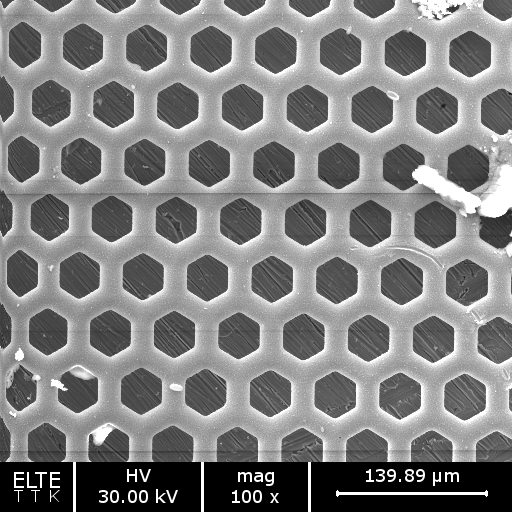
\includegraphics[width=0.8\textwidth]{{img_src/001_a}.png}
    \captionof{figure}{Surface of a microscopic copper grid with 100x magnitude by detecting secondary electrons.} \label{fig:1}
\end{center}
\begin{center}
    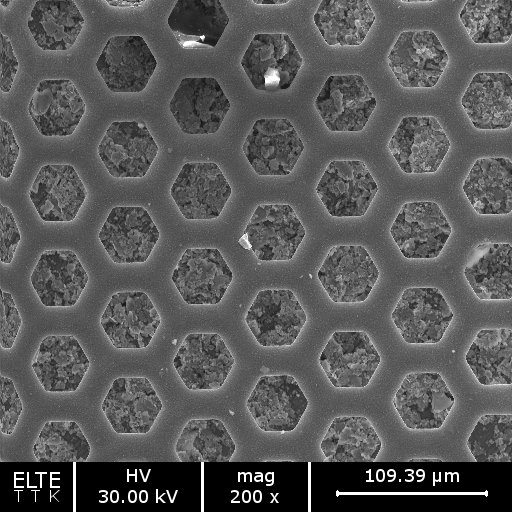
\includegraphics[width=0.8\textwidth]{{img_src/004_a}.png}
    \captionof{figure}{Surface of a microscopic copper grid with 200x magnitude by detecting secondary electrons.} \label{fig:2}
\end{center}
\vspace*{\fill}
\newpage
\topskip0pt
\vspace*{\fill}
\begin{center}
    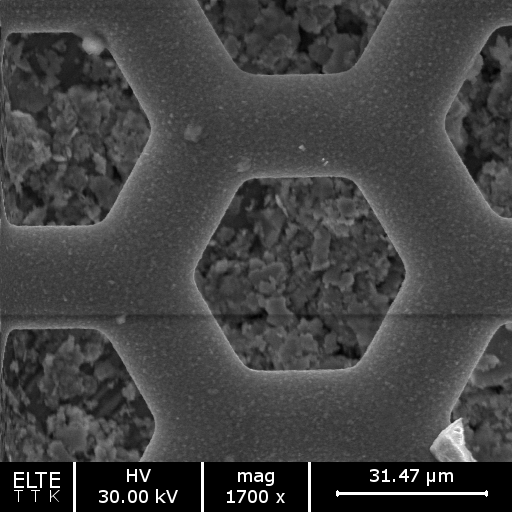
\includegraphics[width=0.8\textwidth]{{img_src/003_a}.png}
    \captionof{figure}{Surface of a microscopic copper grid with 700x magnitude by detecting secondary electrons.} \label{fig:3}
\end{center}
\begin{center}
    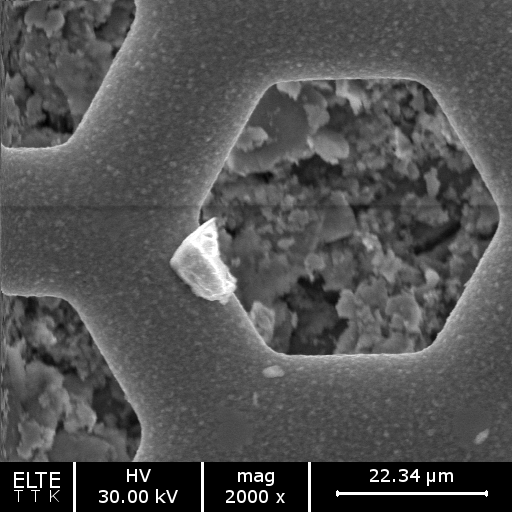
\includegraphics[width=0.8\textwidth]{{img_src/002_a}.png}
    \captionof{figure}{Surface of a microscopic copper grid with 2000x magnitude by detecting secondary electrons. On the copper grid also some contamination could be seen.} \label{fig:4}
\end{center}
\vspace*{\fill}
\newpage